%----------------------------------------------------------------------------------------
%	PACKAGES AND OTHER DOCUMENT CONFIGURATIONS
%----------------------------------------------------------------------------------------

\documentclass{article}
\usepackage{xeCJK} %调用 xeCJK 宏包
\setCJKmainfont{STFangsong} %设置 CJK 主字体为 SimSun (宋体)
\usepackage{fancyhdr} % Required for custom headers
\usepackage{lastpage} % Required to determine the last page for the footer
\usepackage{extramarks} % Required for headers and footers
\usepackage[usenames,dvipsnames]{color} % Required for custom colors
\usepackage{graphicx} % Required to insert images
\usepackage{listings} % Required for insertion of code
\usepackage{courier} % Required for the courier font
\usepackage{lipsum} % Used for inserting dummy 'Lorem ipsum' text into the template
\usepackage{booktabs}
\usepackage{multirow}

% Margins
\topmargin=-0.45in
\evensidemargin=0in
\oddsidemargin=0in
\textwidth=6.5in
\textheight=9.0in
\headsep=0.25in

\linespread{1.1} % Line spacing

% Set up the header and footer
\pagestyle{fancy}
\lhead{\hmwkAuthorName\ \hmwkAuthorNumber} % Top left header
\chead{\hmwkClass\ : \hmwkTitle} % Top center head
\rhead{\firstxmark} % Top right header
\lfoot{\lastxmark} % Bottom left footer
\cfoot{} % Bottom center footer
\rfoot{Page\ \thepage\ of\ \protect\pageref{LastPage}} % Bottom right footer
\renewcommand\headrulewidth{0.4pt} % Size of the header rule
\renewcommand\footrulewidth{0.4pt} % Size of the footer rule

\setlength\parindent{0pt} % Removes all indentation from paragraphs

%----------------------------------------------------------------------------------------
%	CODE INCLUSION CONFIGURATION
%----------------------------------------------------------------------------------------

\definecolor{MyDarkGreen}{rgb}{0.0,0.4,0.0} % This is the color used for comments
\lstloadlanguages{Python} % Load Perl syntax for listings, for a list of other languages supported see: ftp://ftp.tex.ac.uk/tex-archive/macros/latex/contrib/listings/listings.pdf
\lstset{language=Python, % Use Perl in this example
        frame=single, % Single frame around code
        basicstyle=\small\ttfamily, % Use small true type font
        keywordstyle=[1]\color{Blue}\bf, % Perl functions bold and blue
        keywordstyle=[2]\color{Purple}, % Perl function arguments purple
        keywordstyle=[3]\color{Blue}\underbar, % Custom functions underlined and blue
        identifierstyle=, % Nothing special about identifiers                                         
        commentstyle=\usefont{T1}{pcr}{m}{sl}\color{MyDarkGreen}\small, % Comments small dark green courier font
        stringstyle=\color{Purple}, % Strings are purple
        showstringspaces=false, % Don't put marks in string spaces
        tabsize=5, % 5 spaces per tab
        %
        % Put standard Perl functions not included in the default language here
        morekeywords={rand},
        %
        % Put Perl function parameters here
        morekeywords=[2]{on, off, interp},
        %
        % Put user defined functions here
        morekeywords=[3]{test},
       	%
        morecomment=[l][\color{Blue}]{...}, % Line continuation (...) like blue comment
        numbers=left, % Line numbers on left
        firstnumber=1, % Line numbers start with line 1
        numberstyle=\tiny\color{Blue}, % Line numbers are blue and small
        stepnumber=5 % Line numbers go in steps of 5
}

\newcommand{\pythonscript}[2]{
\begin{itemize}
\item[]\lstinputlisting[caption=#2,label=#1]{#1.py}
\end{itemize}
}

%----------------------------------------------------------------------------------------
%	DOCUMENT STRUCTURE COMMANDS
%	Skip this unless you know what you're doing
%----------------------------------------------------------------------------------------

% Header and footer for when a page split occurs within a problem environment
\newcommand{\enterProblemHeader}[1]{
\nobreak\extramarks{#1}{#1 continued on next page\ldots}\nobreak
\nobreak\extramarks{#1 (continued)}{#1 continued on next page\ldots}\nobreak
}

% Header and footer for when a page split occurs between problem environments
\newcommand{\exitProblemHeader}[1]{
\nobreak\extramarks{#1 (continued)}{#1 continued on next page\ldots}\nobreak
\nobreak\extramarks{#1}{}\nobreak
}

\setcounter{secnumdepth}{0} % Removes default section numbers
\newcounter{homeworkProblemCounter} % Creates a counter to keep track of the number of problems

\newcommand{\homeworkProblemName}{}
\newenvironment{homeworkProblem}[1][Problem \arabic{homeworkProblemCounter}]{ % Makes a new environment called homeworkProblem which takes 1 argument (custom name) but the default is "Problem #"
\stepcounter{homeworkProblemCounter} % Increase counter for number of problems
\renewcommand{\homeworkProblemName}{#1} % Assign \homeworkProblemName the name of the problem
\section{\homeworkProblemName} % Make a section in the document with the custom problem count
\enterProblemHeader{\homeworkProblemName} % Header and footer within the environment
}{
\exitProblemHeader{\homeworkProblemName} % Header and footer after the environment
}

\newcommand{\problemAnswer}[1]{ % Defines the problem answer command with the content as the only argument
\noindent\framebox[\columnwidth][c]{\begin{minipage}{0.98\columnwidth}#1\end{minipage}} % Makes the box around the problem answer and puts the content inside
}

\newcommand{\homeworkSectionName}{}
\newenvironment{homeworkSection}[1]{ % New environment for sections within homework problems, takes 1 argument - the name of the section
\renewcommand{\homeworkSectionName}{#1} % Assign \homeworkSectionName to the name of the section from the environment argument
\subsection{\homeworkSectionName} % Make a subsection with the custom name of the subsection
\enterProblemHeader{\homeworkProblemName\ [\homeworkSectionName]} % Header and footer within the environment
}{
\enterProblemHeader{\homeworkProblemName} % Header and footer after the environment
}

%----------------------------------------------------------------------------------------
%	NAME AND CLASS SECTION
%----------------------------------------------------------------------------------------

\newcommand{\hmwkTitle}{Assignment\ \#2} % Assignment title
\newcommand{\hmwkClass}{人工智能导论} % Course/class
\newcommand{\hmwkAuthorName}{张知行} % Your name
\newcommand{\hmwkAuthorNumber}{2015012018}

%----------------------------------------------------------------------------------------
%	TITLE PAGE
%----------------------------------------------------------------------------------------

\title{
\vspace{2in}
\textmd{\textbf{\hmwkClass:\ \hmwkTitle}}\\
%\normalsize\vspace{0.1in}\small{Due\ on\ \hmwkDueDate}\\
%\vspace{0.1in}\large{\textit{\hmwkClassInstructor\ \hmwkClassTime}}
\vspace{3in}
}

\author{\textbf{\hmwkAuthorName\ \hmwkAuthorNumber}}
%\textit{\hmwkAuthorNumber}
\date{\today} % Insert date here if you want it to appear below your name

%----------------------------------------------------------------------------------------

\begin{document}

\maketitle

%----------------------------------------------------------------------------------------
%	TABLE OF CONTENTS
%----------------------------------------------------------------------------------------

%\setcounter{tocdepth}{1} % Uncomment this line if you don't want subsections listed in the ToC

\newpage
%\tableofcontents
%\newpage

\begin{homeworkProblem}[ReflexAgent]
	\paragraph{}
	Description: Improve the ReflexAgent in multiAgents.py to play respectably.
	\paragraph{}
	在autograder中的测试结果如图\ref{reflexAgent}。算法中对剩余食物,ghost和ghost的scaredTimer进行计算,得到估计得分,返回估计得分并完成任务。
	
\end{homeworkProblem}

\begin{homeworkProblem}[MinimaxAgent]
	\begin{figure}[ht]
		\centering
		\begin{minipage}[t]{0.4\textwidth}
		\centering
		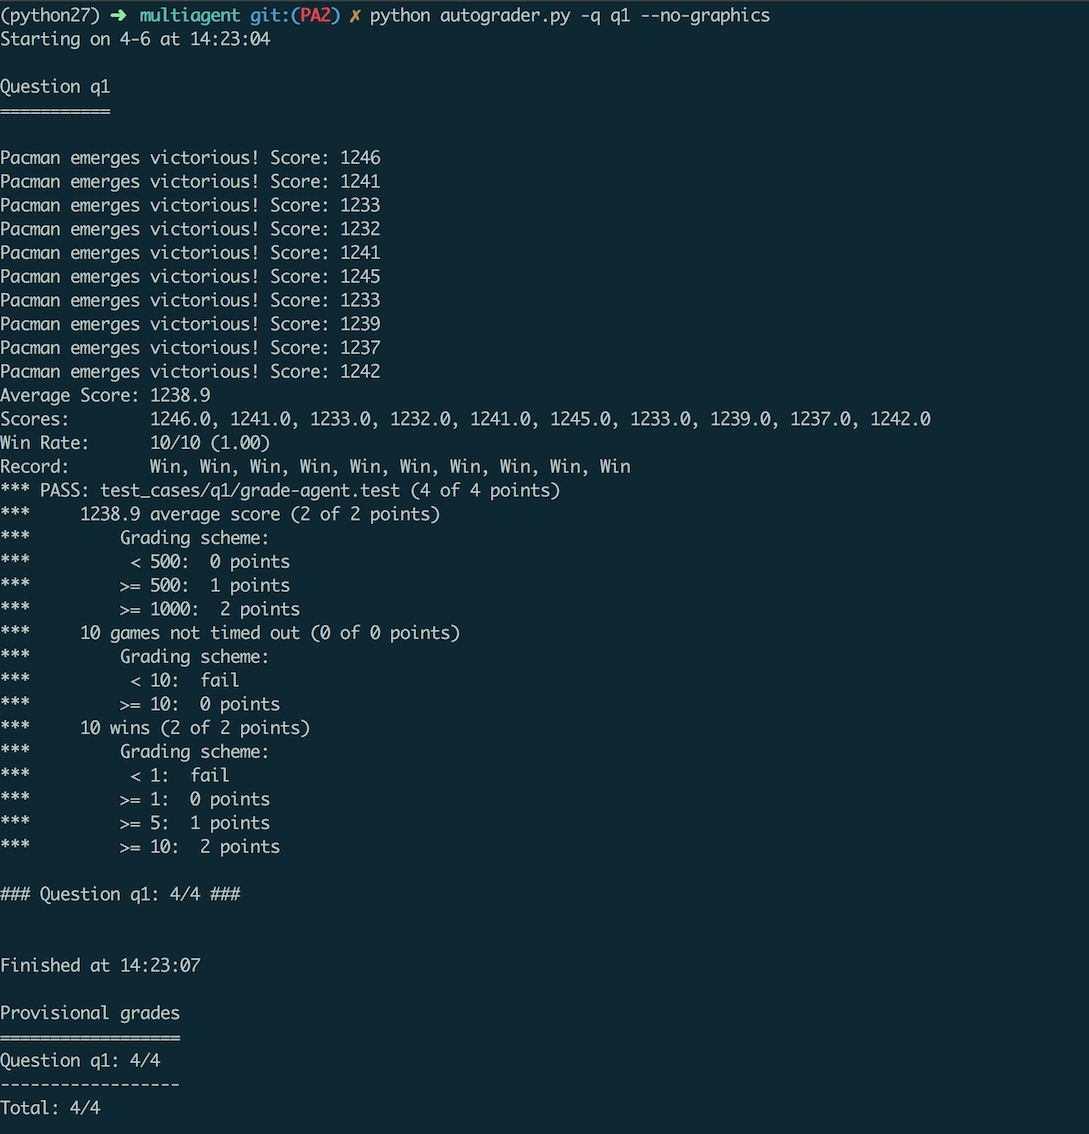
\includegraphics[width=6cm]{q_1.png}
		\caption{ReflexAgent autograder}
		\label{reflexAgent}
		\end{minipage}
		\centering
		\begin{minipage}[t]{0.4\textwidth}
		\centering
		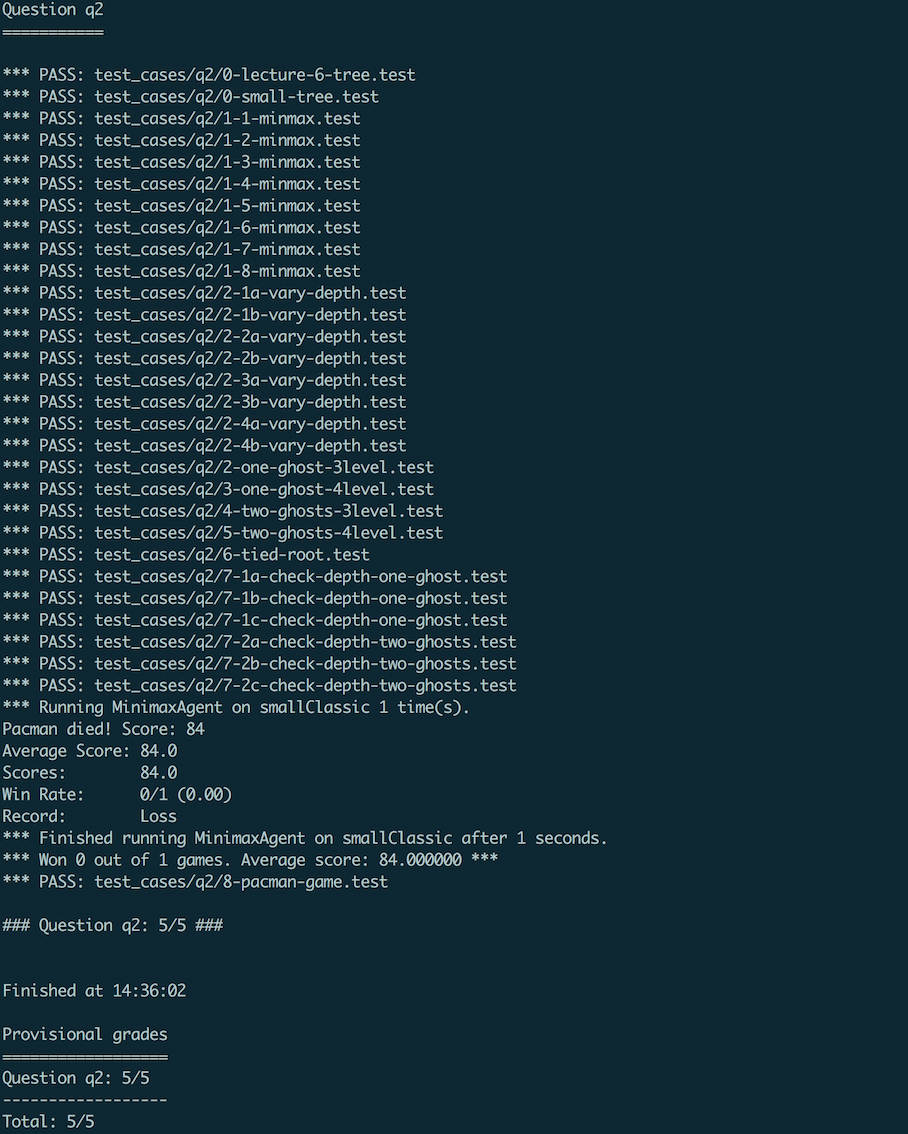
\includegraphics[width=6cm]{q_2.png}
		\caption{MinimaxAgent autograder}
		\label{minimaxAgent}
		\end{minipage}
		\centering
		\begin{minipage}[t]{0.4\textwidth}
		\centering
		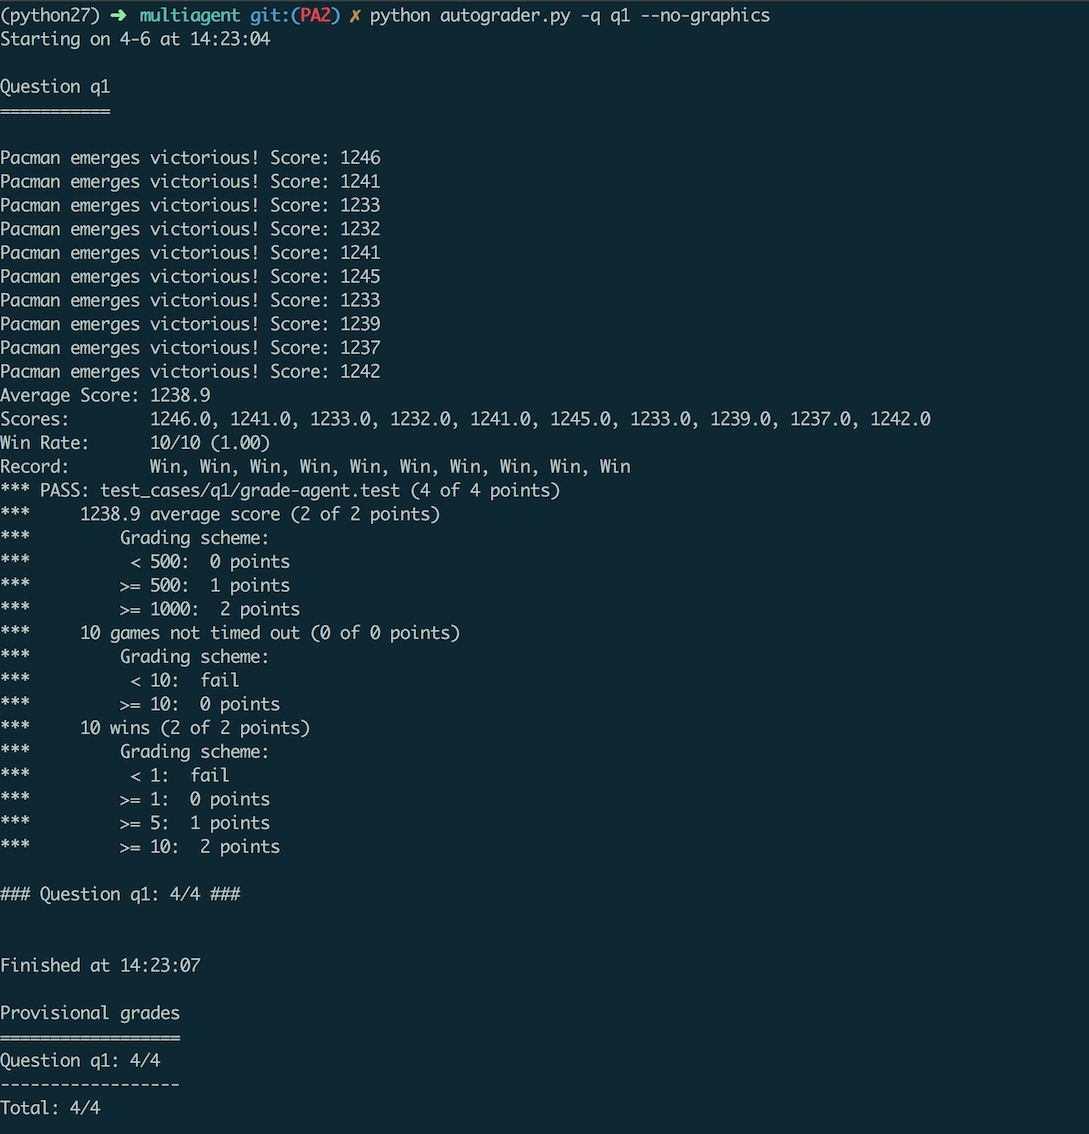
\includegraphics[width=6cm]{q_1.png}
		\caption{AlphaBetaAgent autograder}
		\label{alphabetaAgent}
		\end{minipage}
		\begin{minipage}[t]{0.4\textwidth}
		\centering
		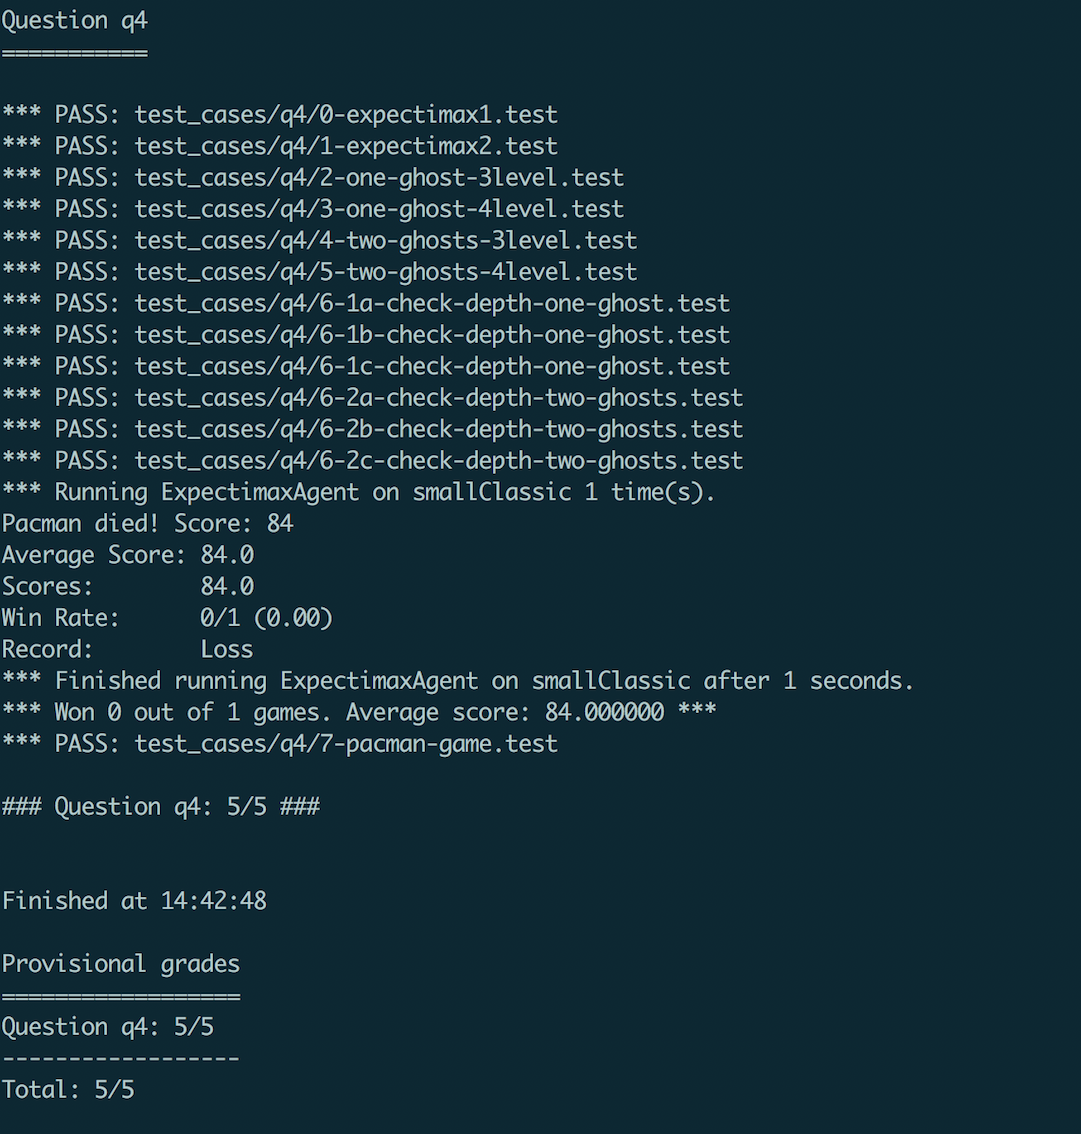
\includegraphics[width=6cm]{q_4.png}
		\caption{ExpectimaxAgent autograder}
		\label{ExpectimaxAgent}
		\end{minipage}
	\end{figure}
	\paragraph{}
	Description: Write an adversarial search agent in the provided MinimaxAgent class stub in multiAgents.py.
	\paragraph{}
	这一问中需要实现minimax算法对PacMan之后行为进行规划,算法中需要考虑到迭代次数,深度以及agents的数目,这一点和PPT中伪代码有所不同,因此将分别针对PacMan和Ghost的Max和Min函数放在一个函数中,同时根据迭代次数进行深度和agent的判断。实现算法的测试结果如图\ref{minimaxAgent}。
	\paragraph{}
	由于在进行对对手的估计时,miniMax算法估计对手的最好情况,因此在进行地图测试时,存在一定可能的情况PacMan失败。同时,在图形界面进行测试的时候,可以发现存在一定的情况PacMan选择在一个地方停止移动,直到ghost来到PacMan附近的时候才可以驱动PacMan进行移动。如果强行修改代码除去PacMan停止不动的操作,可以发现在一定情况下,PacMan更快死亡。
	
\end{homeworkProblem}

\begin{homeworkProblem}[AlphaBetaAgent]
	
	\paragraph{}
	Description: Make a new agent that uses alpha­beta pruning to more efficiently explore the minimax tree, in AlphaBetaAgent.
	\paragraph{}
	这一问中需要在minimax的基础上进行剪枝的操作,只需要简单对minimax函数进行修改,在函数参数传递中传递$\alpha$ 和$\beta$,之后在选取时多一步判断即可完成剪枝操作。这一问在autograder中的测试结果如图\ref{alphabetaAgent}。经过测试,由于展开节点数目减少,alphaBeta剪枝算法同一深度进行搜索可以比MiniMax算法省略一定的时间。
	\paragraph{}
	但是,仍然可以发现,存在一定的情况由于对对方进行过高的估计,PacMan在一些地图上仍然会出现死亡或者停滞不前的情况。对于停止不动的情况可以通过算法中修改对PacMan的legalAction的筛选进行实现,但是在这种情况下,也存在PacMan死亡的情况。
\end{homeworkProblem}

\begin{homeworkProblem}[ExpectimaxAgent]
	\paragraph{}
	Description: Implement the ExpectimaxAgent.
	\paragraph{}
	这一问中使用一个期望值来对对手的选择进行估计,整体上算法实现和minimax中的实现相似,唯一的区别在于对ghost的agents进行估计时,将选择其中的最小值改变为返回其各种选择得分的平均值。使用autograder进行测试的结果如图\ref{ExpectimaxAgent}。这样可以较为合理地估计ghost的行为,从而成功率可能有一定的提升。但是计算量和minimax算法相当,大于alphabeta剪枝算法。
\end{homeworkProblem}
\newpage
\begin{homeworkProblem}[Bonus: Better Evaluation Function]
	\paragraph{}
	Description: Write a better evaluation function for pacman in the provided function betterEvaluationFunction.
	
	\begin{figure}[ht]
		\centering 
		\begin{minipage}[t]{0.4\textwidth}
		\centering
			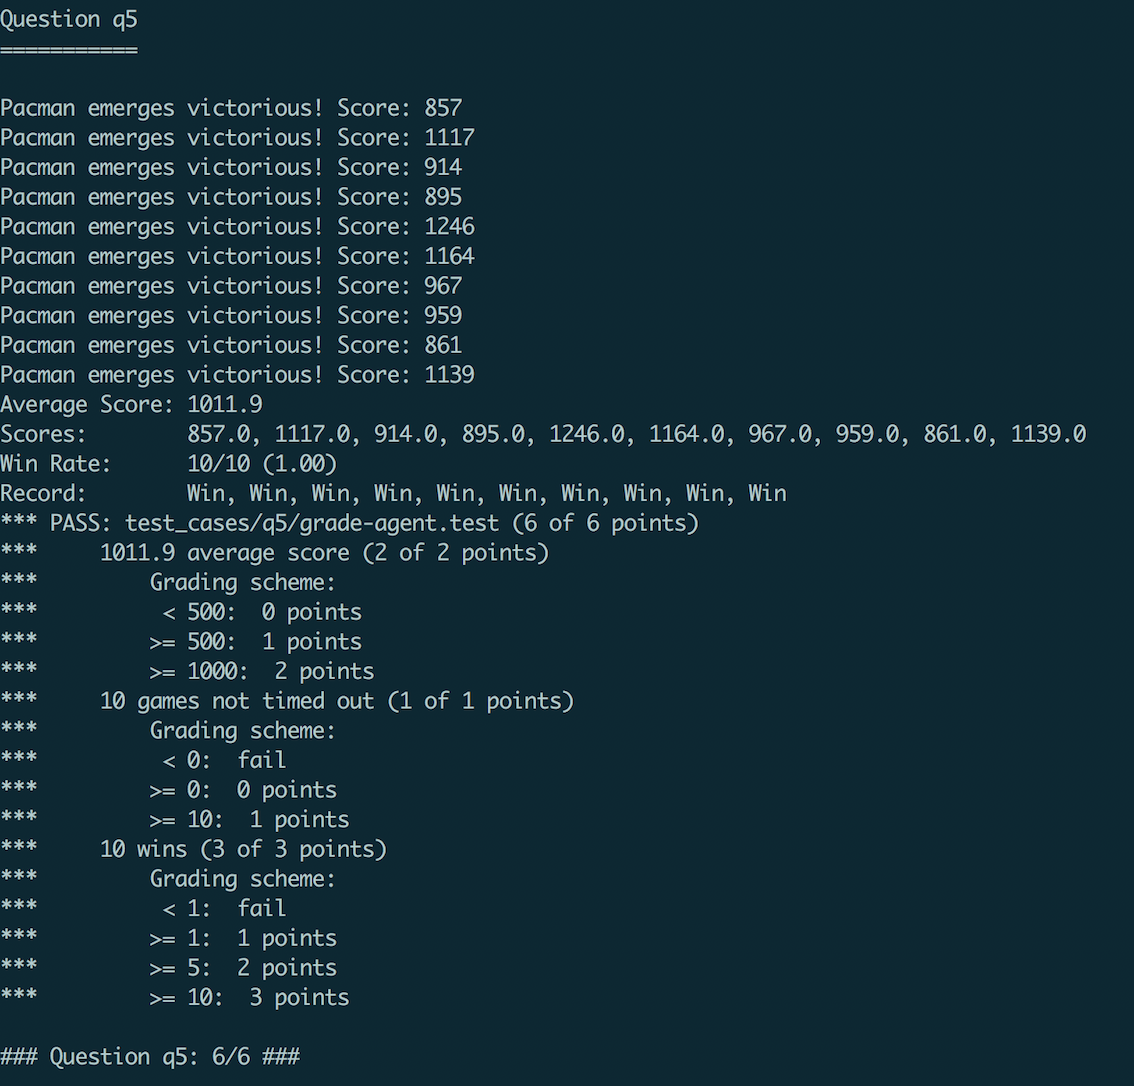
\includegraphics[width=6cm]{q_5.png}
			\caption{Evaluation Function autograder performance}
			\label{eval_func}
		\end{minipage}
		
	\end{figure}
	\paragraph{}
	这一问需要利用当前状态进行评分,由于评分函数影响PacMan对之后的选择,可以考虑ghost,food,scaredtime等进行评估。使用ghost和scaredtime结合进行评估可以较好地实现任务,测试结果如图\ref{eval_func}。使用ghost进行评估标准时,可以有效避免游戏失败,但是由于ghost是驱动PacMan前进的唯一标准,这种评估方式的缺陷是:如果ghost在距离PacMan较远的位置运动,那么PacMan可能选择停止前进,同时,缺乏快速完成所有吃豆工作的动力。但是简单将food通过线性组合考虑进去之后,存在很大的不稳定性,在一些测试条件下会出现失败的情况,而且对选取的参数的要求较高。
	
	
\end{homeworkProblem}

\end{document}